\documentclass[a4paper]{article}
\usepackage[a4paper,%
    text={180mm, 260mm},%
    left=15mm, top=15mm]{geometry}
\usepackage[utf8]{inputenc}
\usepackage{cmap}
\usepackage[english, russian]{babel}
\usepackage{indentfirst}
\usepackage{amssymb}
\usepackage{amsmath}
\usepackage{mathtools}
\usepackage{tcolorbox}
\usepackage{graphicx}
\graphicspath{ { ./figures/ } }

\begin{document}
\title{УМФ. Лекция}
\author{Does not matter}
\maketitle

\begin{equation}
    u_{tt}(x,t) - a^2 u_{xx}(x,t) = 0
    \label{eq:1}
\end{equation}

\textbf{Корректность по Адамару:}\\
Задача математической физики называется корректно поставленной по Адамару, если
решение этой задачи существует в некотором классе ф-й М, определяется в М 
ед. образом и непрерывно зависит от данных задачи

\begin{equation}
    u(x,t) |_{t=0} = \phi(x)
\end{equation}

\begin{equation}
    u_{t}(x,t) |_{t=0} = \psi(x)
\end{equation}
\[
    x \in \mathbb{R}, \; t \geq 0
\]

Вопрос с экза: Формула Даламбера для решения Задачи Коши
\[
    (\theta_{t})^2 - a^2(\theta_{x})^2 = 0 \quad \theta = \theta(x,t)
\]
\[
    \begin{cases}
        \theta_{t} - a \theta_{x} &= 0\\
        \theta_{t} + a \theta_{x} &= 0\\
    \end{cases}
\]
\[
    \begin{cases}
        \frac{dt}{1} &= \frac{dx}{-a} \\
        \frac{dt}{1} &= \frac{dx}{a} \\
    \end{cases}
\]
\[
    \begin{cases}
        x + at &= C_1 \\
        x - at &= C_2 \\
    \end{cases}
\]
\[
    \begin{cases}
        \xi &= x - at \\
        \eta &= x + at 
    \end{cases}
\]
\[
    \tilde{u}_{\xi\eta}(\xi, \eta) = 0
\]
\[
    \frac{\partial}{\partial \xi} (\tilde{u}_{\eta}(\xi, \eta)) = 0
\]
\[
    \tilde{u}_{\eta}(\xi,\eta) = C(\eta)
\]
\[
    \tilde{u}(\xi,\eta) = \int C(\eta)d\eta + f(\xi) \quad \int C(\eta)d\eta = g(\eta)
\]
\begin{equation}
    \tilde{u}(\xi,\eta) = f(\xi) + g(\eta)
\end{equation}
Общее решения ур-я $ (\ref{eq:1}) $: 
\begin{equation}
    u(x,t) = f(x-at) + g(x+at)
\end{equation}
\begin{equation}
    f(x) + g(x) = \phi(x)   
\end{equation}

\begin{figure}[!htb]
    \centering
    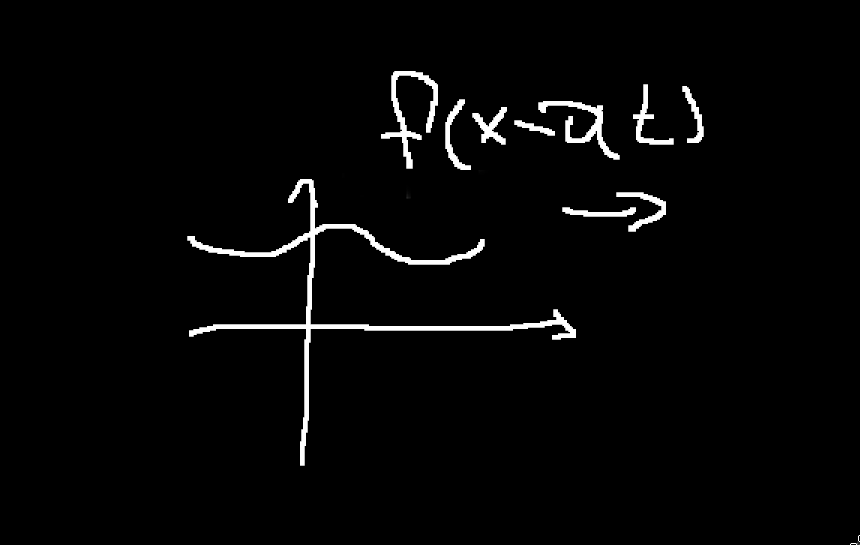
\includegraphics[scale=0.5]{figures/mp-lec-4-10-fig1.png}
    \caption{}
\end{figure}

\[
    -f'(x) + g'(x) = \frac{1}{a} \psi(x)
\]
\[
    u_{t} = f'(x-at) \cdot (x - at)_{t} + g'(x+at) (x+at)_{t} \quad (x+at) = a
\]
\[
    -\int_{x_0}^{x} f'(\chi)d\chi + \int_{x_0}^{x} g'(\chi)d\chi = 
    \frac{1}{a} \int_{x_0}^{x} \psi(\chi)d\chi
\]
\begin{equation}
    -f(x) + g(x) = \frac{1}{a} \int_{x_0}^{x} \psi(\chi)d\chi + C
\end{equation}
\[
    g(x) = \frac{1}{2a} \int_{x_0}^{x} \psi(\chi)d\chi + \frac{\phi(x)}{2} + \frac{C}{2} 
\]
\[
    f(x) = \frac{-1}{2a} \int_{x_0}^{x} \psi(\chi)d\chi + \frac{\phi(x)}{2} - \frac{C}{2} 
\]
\[
    u(x,t) = \frac{\phi(x-at)+\phi(x+at)}{2} + \frac{1}{2a} 
    \int_{x_0}^{x+at} \psi(\chi)d\chi - \frac{1}{2a} \int_{x_0}^{x-at}\psi(\chi)d\chi 
\]
\[
    u(x,t) = \frac{\phi(x-at)+\phi(x+at)}{2} + \frac{1}{2a} 
    \int_{x_0}^{x+at} \psi(\chi)d\chi + \frac{1}{2a} \int_{x-at}^{x_0}\psi(\chi)d\chi 
\]
\begin{equation}
    u(x,t) = \frac{\phi(x-at)+\phi(x+at)}{2} + \frac{1}{2a} 
    \int_{x-at}^{x+at} \psi(\chi)d\chi 
\end{equation}
\[
    u \in C^2(\mathbb{R} \times [0;\infty]) \quad \phi \in C^2(\mathbb{R})
    \quad \psi \in C^{1}(\mathbb{R})
\]

Непрерывная зависимость решения от данных:\\
\[
    u_{tt}^{(i)}(x,t) - a^2 u_{xx}^{(i)}(x,t) = 0
\]
\[
    u^{(i)}(x,t) |_{t=0} = \phi(x)
\]

\[
    u_{t}^{(i)}(x,t) |_{t=0} = \psi(x)
\]
\[
    u = u^{(1)} - u^{(2)}
\]
\[
    \phi = \phi^{(1)} - \phi^{(2)}
\]
\[
    \psi = \psi^{(1)} - \psi^{(2)}
\]
\[
    |u(x,t)| \leq \frac{|\phi(x-at)|+|\phi(x+at)|}{2} + \frac{1}{2a} 
    \int_{x-at}^{x+at} |\psi(\chi)| d\chi \leq \epsilon + \frac{\delta}{2a} \cdot
    2aT = \epsilon + \delta T
\]
\[
    0 \leq t \leq T
\]
\[
    | \phi^{(1)} - \phi^{(2)} | \leq \epsilon
\]
\[
    | \psi^{(1)} - \psi^{(2)} | \leq \delta
\]
\[
    |u^{(1)} - u^{(2)}| \leq \delta + \delta T \rightarrow 0
\]
\[
    x \in \mathbb{R}, \; t \in [0,T]
\]
\begin{figure}[!htb]
    \centering
    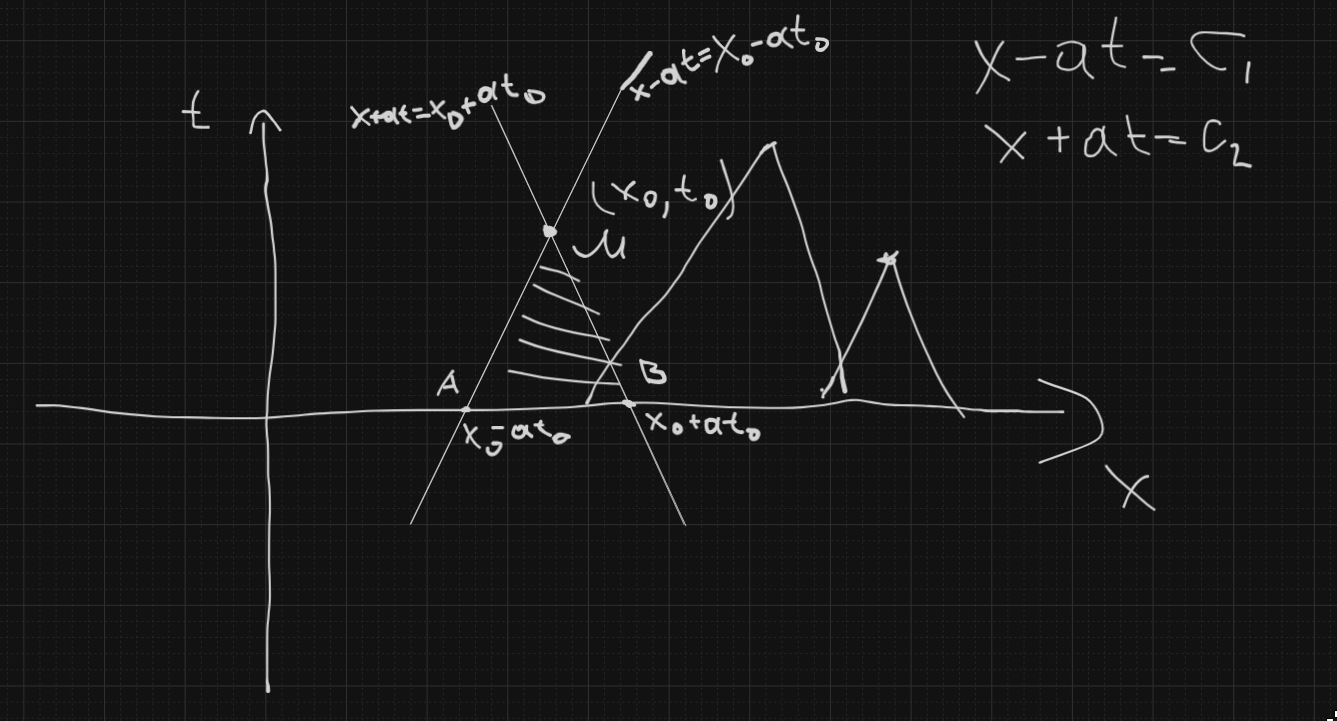
\includegraphics[scale=0.3]{figures/mp-lec4-10-fig2.png}
    \caption{Характеристический треугольник}
\end{figure}

Характеристический треугольник AMB называется область определённости

Вопрос из экза:\\
Свободные колебания полубесконечной струны с закреплённым концом

\begin{figure}[!htb]
    \centering
    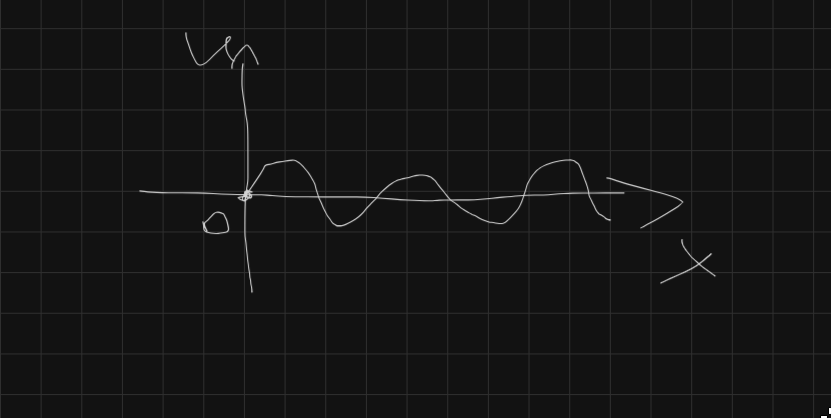
\includegraphics[scale=0.3]{figures/mp-lec4-10-fig3.png}
\end{figure}

Для ур-я $ (\ref{eq:1}) $ 
\[
    x \geq 0, \; t \geq 0
\]
\[
    u_{tt}(x,t) - a^2 u_{xx}(x,t) = 0
\]
\[
    u(x,t) |_{t=0} = \phi(x)
\]

\[
    u_{t}(x,t) |_{t=0} = \psi(x)
\]
Также:
\[
    u(0,t) = 0
\]
\[
    U_{tt}(x,t) - a^2U_{xx}(x,t) = 0, \; t \geq 0,\; x \in \mathbb{R}
\]
\[
    V(x,t)|_{t=0} = \Phi(x), \; x \in \mathbb{R}
\]
\[
    V_{t}(x,t)|_{t=0} = \Psi(x), \; x \in \mathbb{R}
\]
\[
    \Phi(x) = \begin{cases}
        \phi(x), &\quad x \geq 0\\
        -\phi(-x), &\quad x \leq 0
    \end{cases}
\]
\[
    \Psi(x) = \begin{cases}
        \psi(x), &\quad x \geq 0\\
        -\psi(-x), &\quad x \leq 0
    \end{cases}
\]
\[
    (\phi(0) = 0, \psi(0) = 0 \text{ - условия согласования})
\]
\[
    U(x,t) = \frac{\Phi(x-at)+\Phi(x+at)}{2} + \frac{1}{2a} 
    \int_{x-at}^{x+at} \Psi(\chi)d\chi 
\]
\[
    U(0,t) \equiv 0
\]
\end{document}
